\section{Introduzione}\todo{prima bozza.. ancora da rileggere completamente}

Il seguente progetto ha come obiettivo quello di realizzare un'applicazione che consenta di ricavare automaticamente la rappresentazione in \LaTeX \;di un circuito elettrico realizzato con il software di simulazione LTSpice (\href{https://www.analog.com/en/design-center/design-tools-and-calculators/ltspice-simulator.html}{Analog Devices}). In particolare, il pacchetto \href{https://it.overleaf.com/learn/latex/CircuiTikz_package}{CircuiTikz} permette di rappresentare in Latex un circuito elettrico. Inoltre, LTSpice produce un file con estensione .asc che contiene tutte le informazioni utili alla rappresentazione grafica dei componenti, come ad esempio la posizione assoluta dei vari elementi circuitali, la loro etichetta e il loro valore. L'idea alla base di questo progetto è quella di utilizzare le informazioni contenute nel file .asc e il pacchetto CircuiTikz per ottenere una rappresentazione in Latex del circuito. Una volta ottenuto il file .tex, si utilizza lo strumento \texttt{pdflatex} (distribuito con il compilatore MikTex) per generare un documento pdf.
\subsection{Tecnologie utilizzate}
Per lo sviluppo di questo progetto si sono utilizzate le seguenti tecnologie:
\begin{itemize}
	\item \texttt{ANTLRWorks 1.5.2}, per la generazione del lexer e del parser nel linguaggio java;
	\item libreria java \texttt{antlr-complete} versione 3.4;
	\item libreria \texttt{CircuiTikz} e il compilatore \texttt{MikTex}, per la generazione del codice Latex e del documento pdf;
	\item \texttt{Eclipse IDE}, per la creazione del progetto java del lexer e del parser e la compilazione;
	\item framework Qt, per la creazione dell'app client;
	\item \texttt{GitHub}, per il versioning del codice;
\end{itemize}
\subsection{LTSpice}
LTSpice è un software molto utilizzato in ambito accademico e lavorativo per effettuare simulazione di circuiti elettrici. L'interazione con il programma avviene tramite un'interfaccia grafica che permette di inserire i componenti, assegnare loro un valore e un identificativo e definire i parametri di simulazione (\Fig\ref{fig:ltspice}).
\begin{figure}[h!]
	\centering
	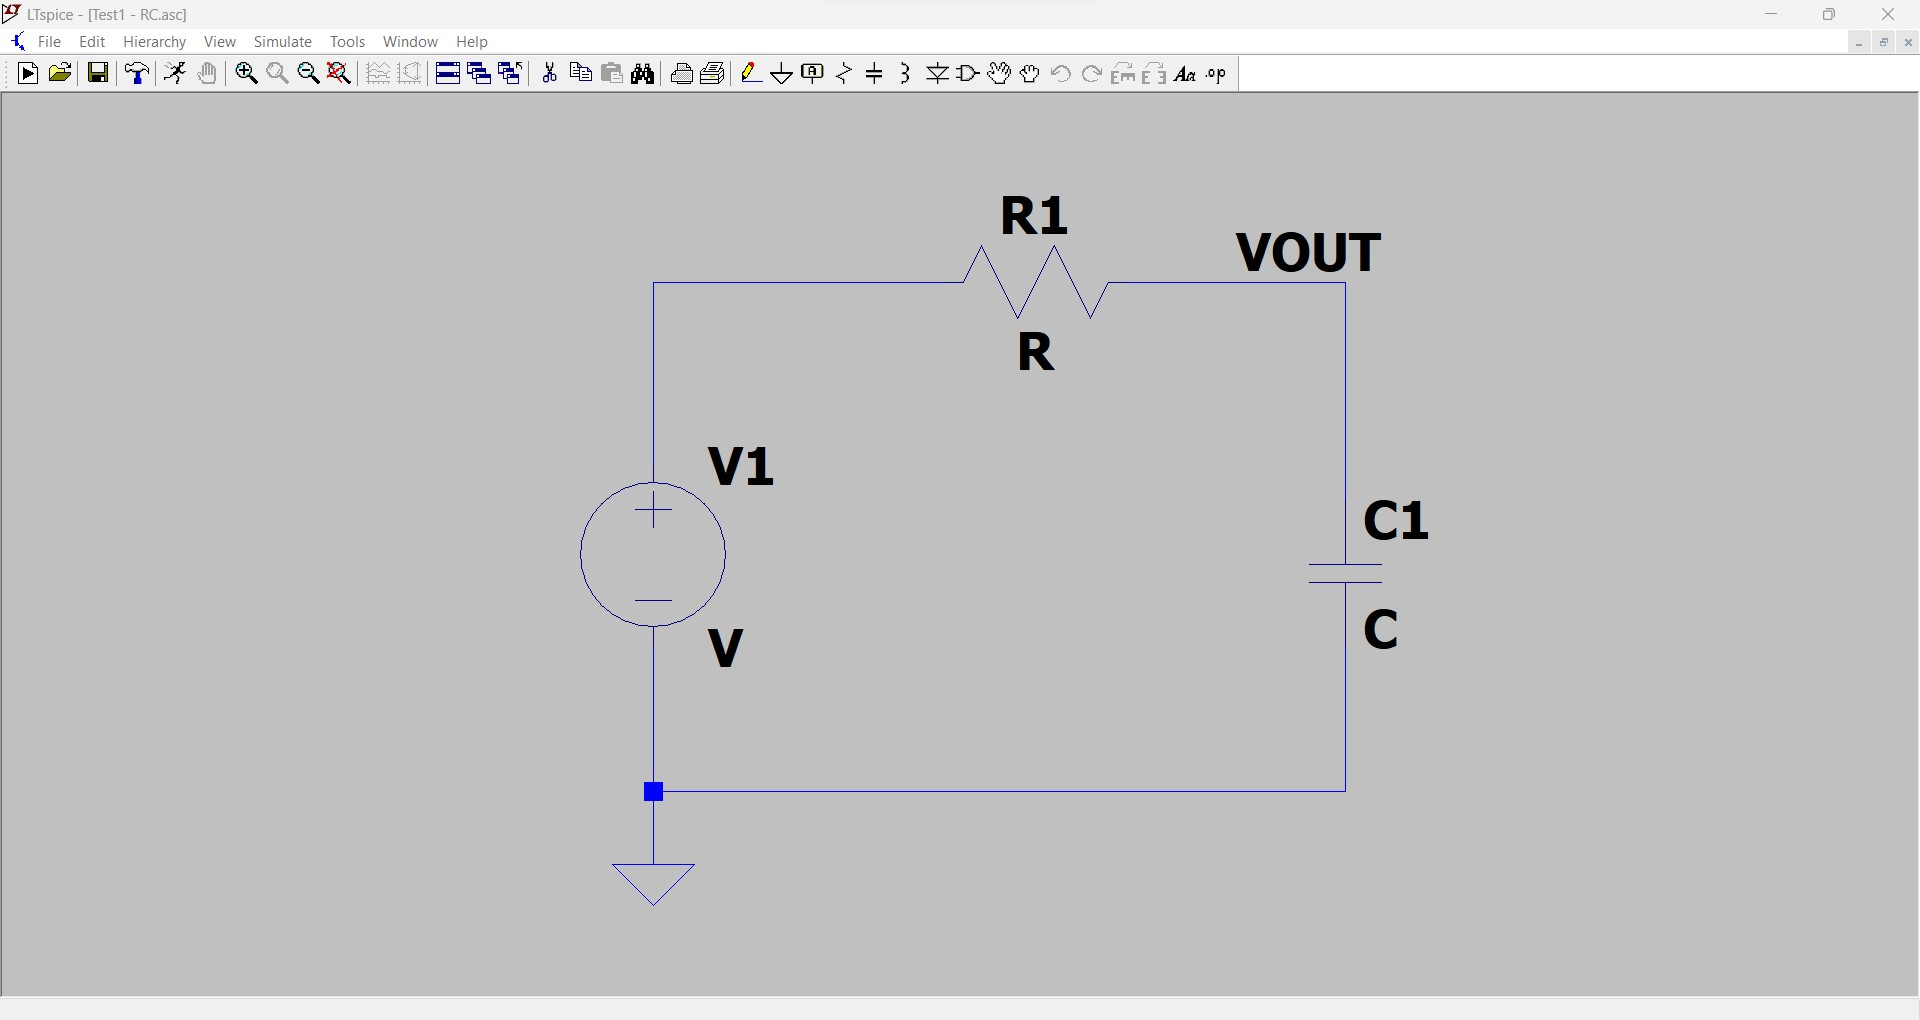
\includegraphics[width=\textwidth]{./ImageFiles/LTSpice.jpg}
	\caption{Schermata principale di LTSpice.}
	\label{fig:ltspice}
\end{figure}
Il motore di simulazione è basato sul programma SPICE (\textit{Simulation Program with Integrated Circuit Emphasis}) che riceve in input una \texttt{netlist}, ossia una rappresentazione testuale del circuito, e produce in output i risultati di simulazione. LTSpice crea automaticamente la \texttt{netlist} a partire dalla rappresentazione grafica del circuito. Per esempio, il circuito in figura \ref{fig:ltspice} genera la seguente netlist:
\lstinputlisting[language=Octave]{./OtherFiles/netlist.txt}
Inoltre, il programma salva il circuito in un file con estensione .asc che contiene tutte le informazioni per rappresentare in modo grafico il circuito. Di seguito si riporta il file .asc prodotto dal circuito in figura \ref{fig:ltspice}.
\lstinputlisting[language=Octave]{./OtherFiles/asc.txt}
Come si può notare, in questo file non vengono riportate informazioni sulla simulazione da eseguire ma bensì la posizione dei collegamenti e dei componenti, la posizione di label associate ed eventuali attributi. In particolare, le principali parole chiave che si possono riconoscere sono: \todo{descrizione generica. c'è dopo la grammatica}
\begin{itemize}
	\item VERSION, rappresenta la versione del sistema utilizzato\todo{non è la versione di ltspice}; per il progetto verrà considerata solamente la versione 4;
	\item SHEET, definisce il numero del figlio di lavoro utilizzato e le relative dimensioni;
	\item WIRE, indica un filo di collegamento; seguono le coordinate x,y assolute dei relativi capi;
	\item SYMBOL, rappresenta un componente; viene indicato di seguito la tipologia, la posizione assoluta in coordinate x,y e l'eventuale rotazione o mirror; è possibile indicare una rotazione di 0°, 90°, 180°, 270° o un'operazione di mirror di 0°, 90°, 180° e 270°;
	\item SYMATTR, permette di indicare eventuali attributi riferiti a un simbolo come il nome, il valore, i parametri di eventuali componenti parassiti o indicare il produttore del componente;
	\item WINDOW, indica la posizione della label associata a un componente (il nome o il valore) nel caso di rotazioni e mirror;
	\item FLAG, definisce la posizione e il contenuto di eventuali label associati a dei collegamenti in un circuito; viene utilizzata anche per indicare la massa (indicando come nome della label 0);
	\item IOPIN, indicano label di ingresso o uscita nel circuito. 
\end{itemize}
Tutte le coordinate sono espresse attraverso numeri interi e le parole chiave sono interpretate in modo \textit{case insensitive}. Il formato di codifica del file è \texttt{ISO-8859-1} e accetta qualsiasi carattere \texttt{UNICODE} all'interno delle label e dei nomi dei componenti. Le parole chiave e i relativi parametri sono separati da degli spazi bianchi. LTSpice è insensibile al numero di spazi tra i diversi token e di eventuali \textit{newline}. Tuttavia, il file .asc in output a LTSpice è formattato mantenendo un unico spazio tra ogni token e andando a capo ad ogni parola chiave.

\section{ltspice2circuitikz}

\begin{figure}[h!]
	\centering
	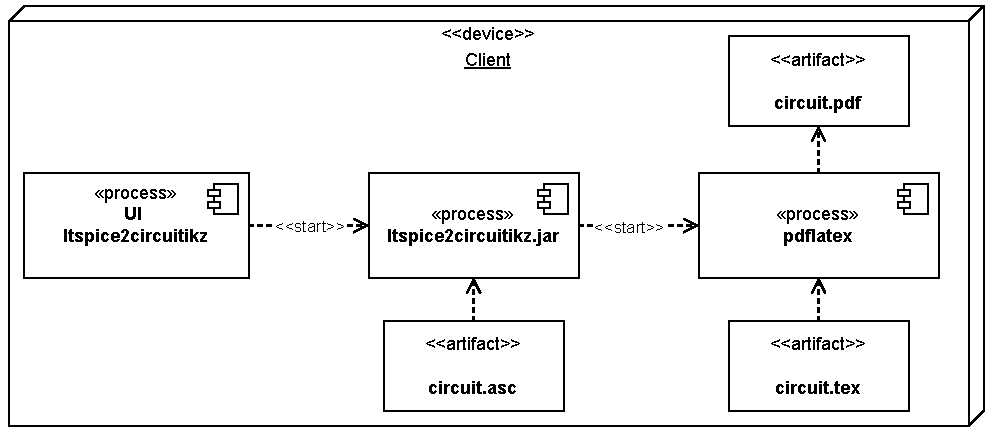
\includegraphics[width=0.5\textwidth]{./ImageFiles/deploy diagram.pdf}
	\caption{Deploy diagram del sistema.}
	\label{fig:deploy_diagram}
\end{figure}


\subsubsection{Lexer e Parser}
L'applicazione realizzata si basa su un lexer e un parser LL(1) generato grazie al tool AntlrWorks, che permette di leggere ed interpretare un file .asc e di effettuare la traduzione in un file .tex, grazie a delle azioni semantiche.

\begin{figure}[h!]
	\centering
	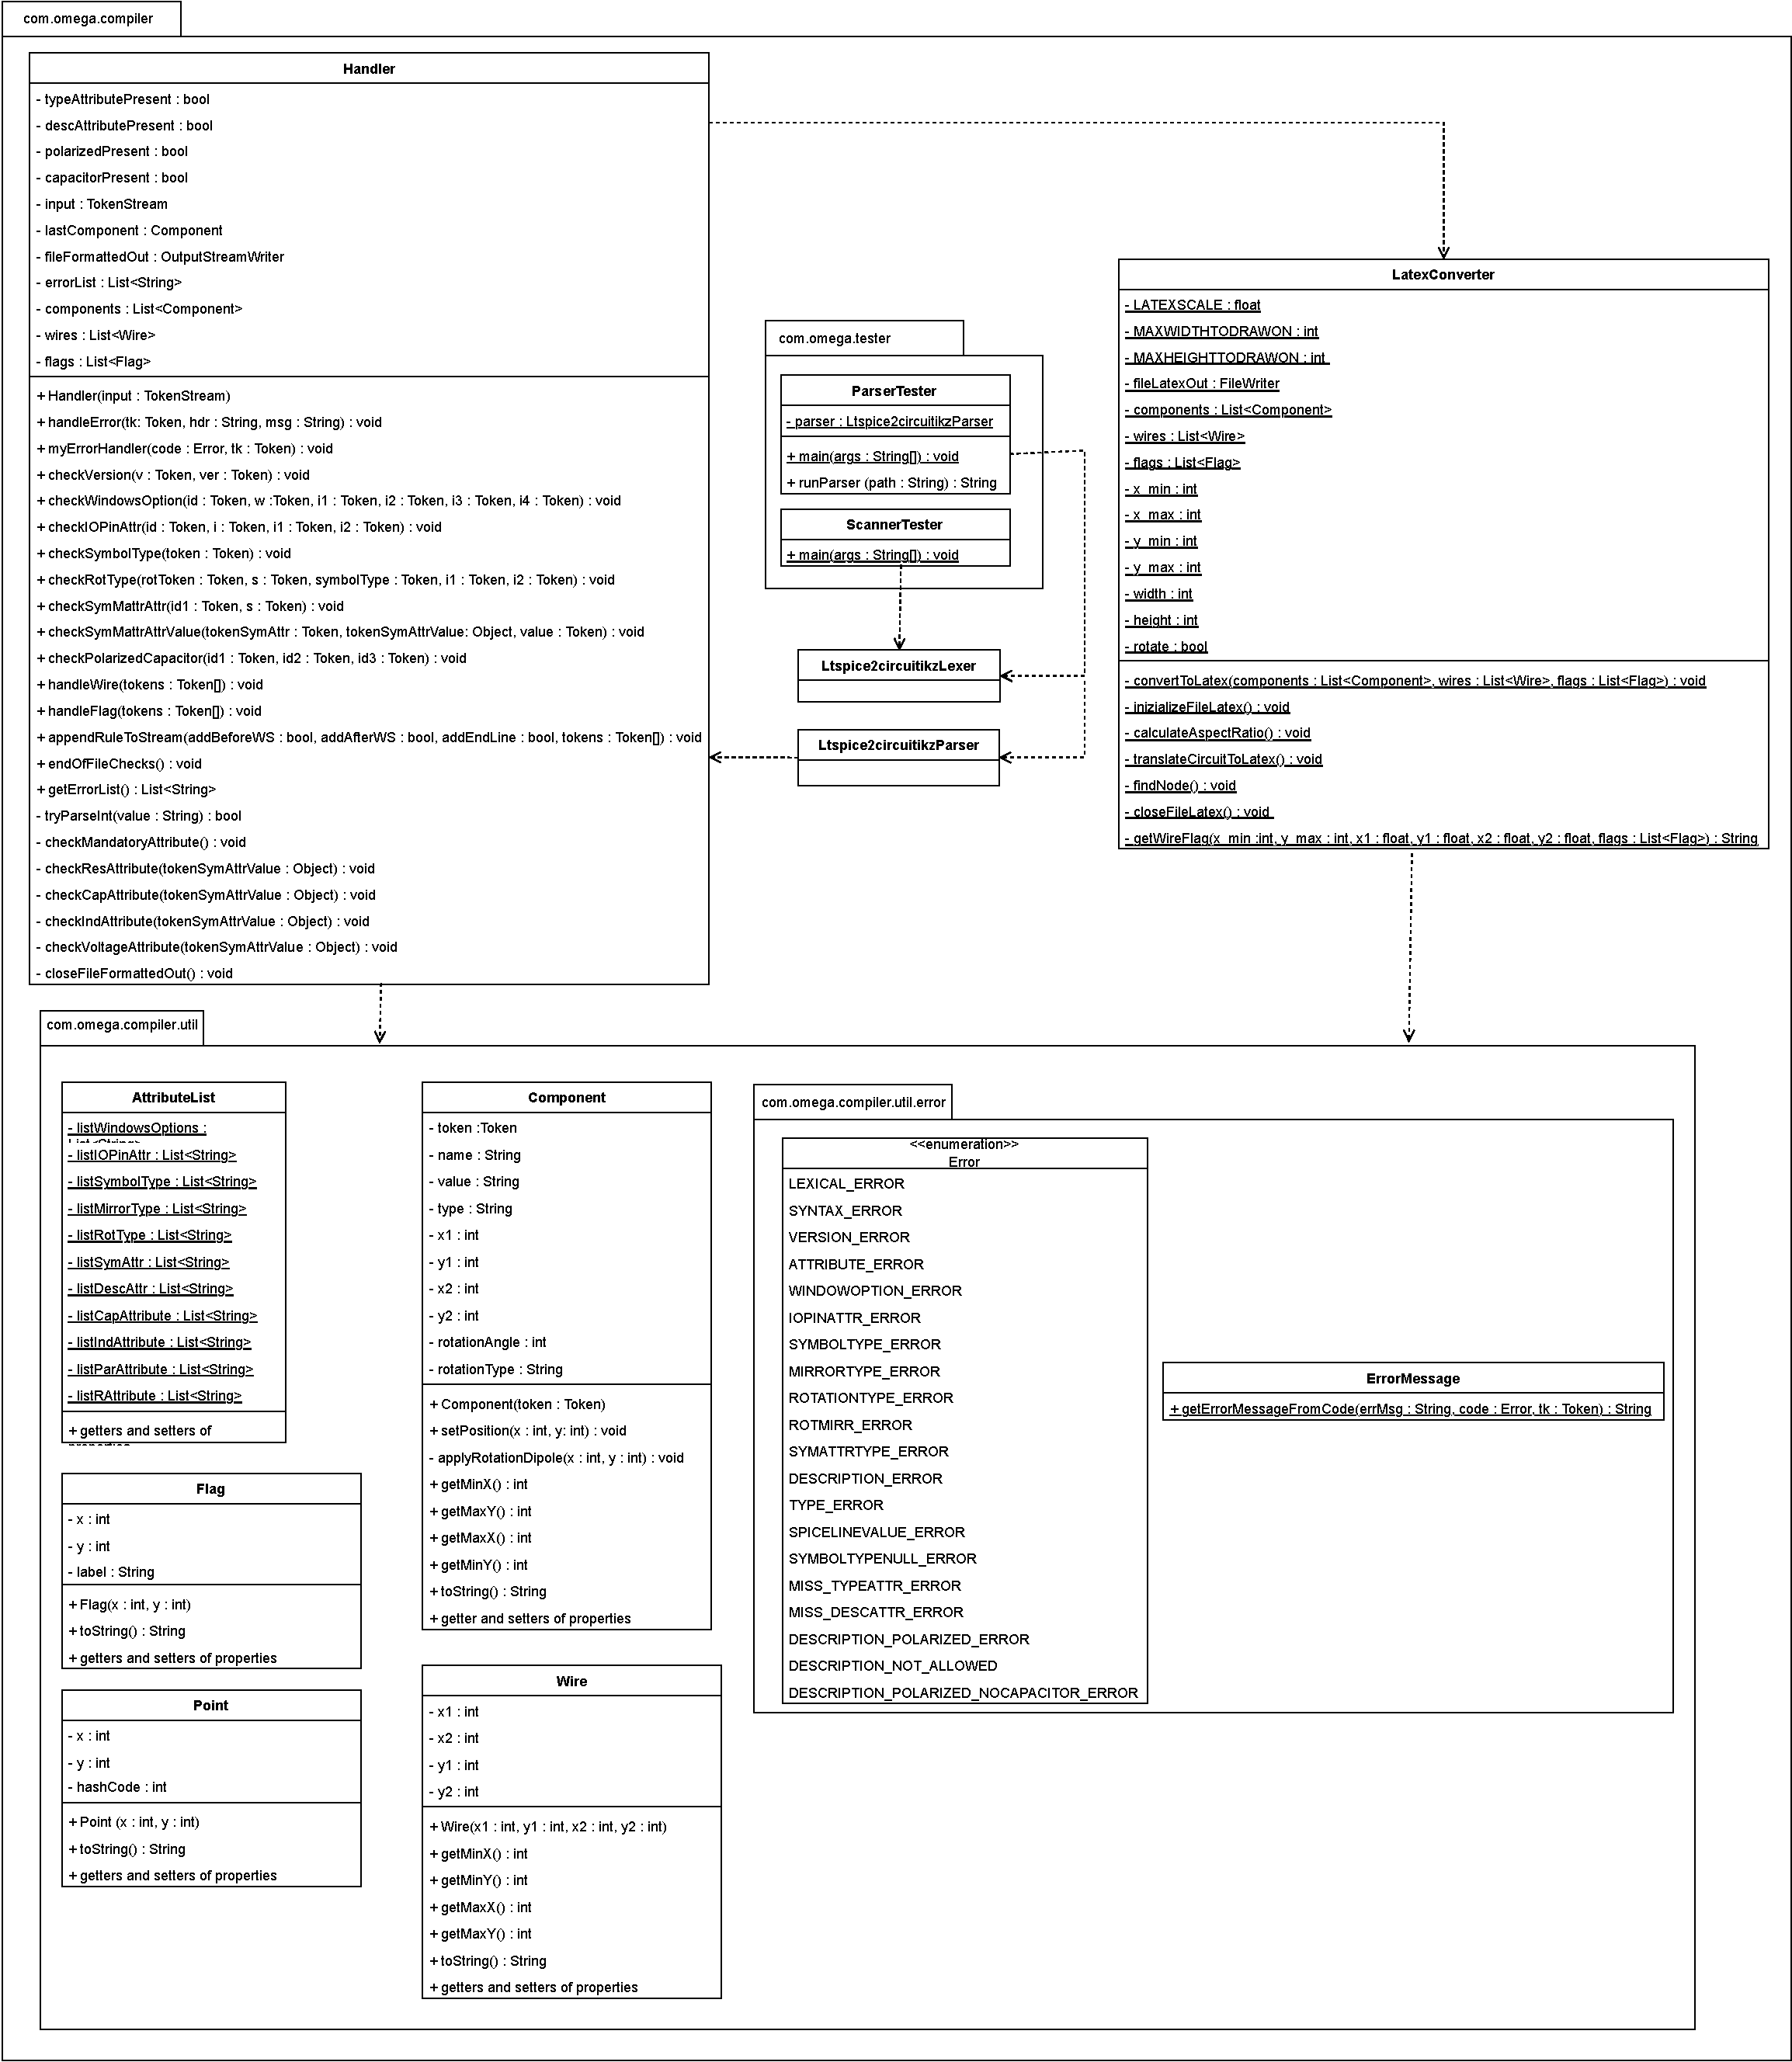
\includegraphics[width=\textwidth]{./ImageFiles/class and package diagram.pdf}
	\caption{Class and Package Diagram dell'applicazione.}
	\label{fig:class_diagram}
\end{figure}